\documentclass[tikz,border=4pt]{standalone}
% Shared style for every figure and for the deck: one accent, one
% highlight, thin lines, rounded nodes, nothing decorative.
\usepackage[T1]{fontenc}
\usepackage{lmodern}
\renewcommand{\familydefault}{\sfdefault}
\usepackage{tikz}
\usetikzlibrary{arrows.meta,positioning,calc,shapes.misc,fit,backgrounds,decorations.pathreplacing}
\definecolor{ink}{RGB}{40,40,40}
\definecolor{soft}{RGB}{150,150,150}
\definecolor{faint}{RGB}{225,225,225}
\definecolor{accent}{RGB}{0,95,115}
\definecolor{accentlight}{RGB}{214,232,236}
\definecolor{warn}{RGB}{196,84,40}
\definecolor{warnlight}{RGB}{247,226,216}
\tikzset{
  every picture/.style={color=ink, line width=0.5pt, font=\small},
  node distance=12mm and 18mm,
  box/.style={draw=ink, rounded corners=2pt, fill=white, inner sep=5pt, minimum height=7mm, align=center},
  maker/.style={box, minimum width=18mm},
  cat/.style={box, inner sep=3.5pt, minimum height=6mm},
  root/.style={box, fill=accentlight, draw=accent},
  bad/.style={box, fill=warnlight, draw=warn},
  ghost/.style={box, draw=soft, text=soft, dashed},
  flow/.style={-{Stealth[length=4pt,width=3.5pt]}, line width=0.5pt},
  sub/.style={-{Stealth[length=4pt,width=3.5pt]}, line width=0.5pt, color=soft},
  strong/.style={flow, color=accent, line width=0.8pt},
  wrong/.style={flow, color=warn},
  lbl/.style={font=\footnotesize, text=ink, inner sep=1.5pt, fill=white},
  note/.style={font=\footnotesize, text=soft, align=center},
  rate/.style={font=\footnotesize, text=accent, inner sep=1pt, fill=white},
}

\usepackage{amsmath}
\usepackage{pgfplots}
\pgfplotsset{compat=1.17}

\begin{document}
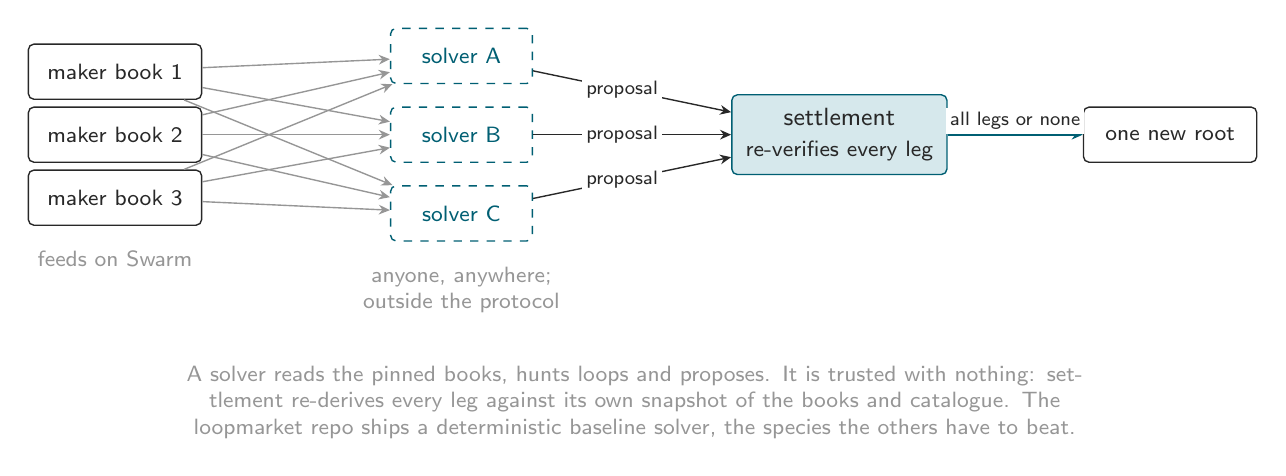
\begin{tikzpicture}
  % Solvers live outside the protocol (the CoW Protocol shape): anyone
  % runs one, they compete, and settlement trusts none of them.
  \foreach \i/\y in {1/8,2/0,3/-8} { \node[box, minimum width=22mm, font=\footnotesize] (b\i) at (0,\y mm) {maker book \i}; }
  \node[note, below=2mm of b3] {feeds on Swarm};
  \foreach \i/\y/\n in {1/10/solver A,2/0/solver B,3/-10/solver C} { \node[maker, dashed, draw=accent, text=accent, font=\footnotesize] (s\i) at (44mm,\y mm) {\n}; }
  \node[note, below=2mm of s3, text width=34mm] {anyone, anywhere; outside the protocol};
  \foreach \i in {1,2,3} \foreach \j in {1,2,3} { \draw[sub] (b\i) -- (s\j); }
  \node[root, minimum width=26mm, align=center] (set) at (92mm,0) {settlement\\{\footnotesize re-verifies every leg}};
  \foreach \i in {1,2,3} { \draw[flow] (s\i) -- node[lbl, pos=0.45, font=\scriptsize] {proposal} (set); }
  \node[box, minimum width=22mm, font=\footnotesize] (root) at (134mm,0) {one new root};
  \draw[strong] (set) -- node[lbl, above, font=\scriptsize] {all legs or none} (root);
  \node[note, text width=120mm] at (66mm,-34mm) {A solver reads the pinned books, hunts loops and proposes. It is trusted with nothing: settlement re-derives every leg against its own snapshot of the books and catalogue. The loopmarket repo ships a deterministic baseline solver, the species the others have to beat.};
\end{tikzpicture}
\end{document}
